\documentclass[a4paper]{article}     
\usepackage{amsfonts}
\usepackage{amsmath}
\usepackage{amssymb}
\usepackage{graphicx}
\newcommand{\dint}{\displaystyle\int}

\begin{document}

\noindent \large Auteur: Michaël Francken \\
\noindent \large Studierichting: Informatica\\
\noindent \large Oefeningenreeks 5D nr.1.3 \\

\medskip

\normalsize

$f(x)=\sqrt[3]{x} $ op het interval [0,8]\\

$f(x)=x^{\tfrac{1}{3}}$\\

$F(x)=\dfrac{x^{\tfrac{1}{3}+1}}{\dfrac{1}{3}+1}$\\

$=\dfrac{3}{4}x^{\tfrac{4}{3}}$\\

$=\left[ \dfrac{3}{4}x^{\tfrac{4}{3}} \right]^8_0$\\

$=\left(\dfrac{3}{4}\cdot 8^{\tfrac{4}{3}}\right)-\left(\dfrac{3}{4}\cdot 0^{\tfrac{4}{3}}\right)$\\

$=\dfrac{3}{4\sqrt[3]{8^4}}=3\cdot 4=12$\\

\begin{figure}[h]
\centering
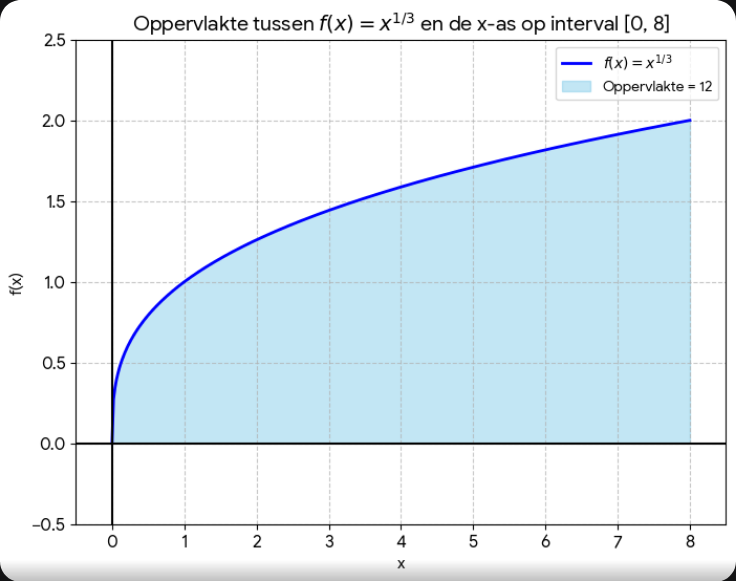
\includegraphics[width=5cm]{5D-1.3-michael.francken.INF.png}
\end{figure}

\begin{thebibliography}{999}
%\bibitem{a} Referentie
\end{thebibliography}
\end{document} 
